\chapter{Development Plan}
\label{chap:Chapter5}
%-------------------------------------------------------------------------------%
\section{Research Approach}
To achieve the desired objectives and system requirements, the development approach will be composed of three phases: Dissertation Development, System Development, and Implementation.

During the first part of dissertation development it will be analyzed the problems with fixed-pitch propeller systems, described in the previous chapters, in \glspl{uav} to be able to find the best approach to solve the issue at hand, to define the new system requirements, determine the objectives of the proposed solution and to design the system architecture.
And, to gain a better understanding of the present status of the subject, a study of the literature on related to the problem, will be conducted.
In this phase, it will be also written all the steps and considerations took during the development and implementation of the solution and an analysis of the results obtained.

As we go on to the System Development phase, there will be a detailed procurement to find the most adequate components, according to the system architecture and requirements, since it is necessary to design and manufacture \glspl{PCB} for the final prototype.
In this phase, the system flow charts, shown in appendix , will be modeled and validated using model checker tools like NuSMV.
This step will increase the confidence in the designed firmware and validate the expected behavior of the system.

In the implementation phase, the Main and Secondary Devices wil be soldered and assembled, to, later on perform, bench and ground tests, and evaluate the developed system in comparison to predetermined goals and requirements.
By documenting and analyzing the results it will be possible to make any necessary refinements to enhance performance.

%-------------------------------------------------------------------------------%

\section{Evaluation}
In order to evaluate the system performance, in comparison to the requirements, the analyses will be divided in three categories.

In the Communication category, it will be analyzed the stability and the latency of the chosen communication technology.

Another category is the Pitch Angle Control in which the precision and stability of the control over the pitch angle will be evaluated.
It will also be analyzed if the system has a quick response to change in flight phase and Maneuver, a quick response in error scenarios and if the fail-safe mechanism is able to set a fixed pitch angle.

The last category to be evaluated is the Firmware.
In this category the model of the system flow will be validated with mathematical tools like explained before.

This way, the system will be evaluated in each subsystem and as a whole.

%-------------------------------------------------------------------------------%

\section{Timeline}
In the Gantt chart (figure \ref{fig:gantt}) all phases, described previously in the Research Approach section, were added together with multiple tasks and subtasks each with a given duration and dependencies.

The first task started is the Research Plan, part of Dissertation Development phase, and will be the starting point of future work.
All the other tasks, in this phase, will be done in parallel until the end of the dissertation.

Next will be the System Development phase were hardware and firmware tasks will be made.
These tasks will start mid January 2024 and end in early April 2024.

The last tasks will be from Implementation phase with tests, evaluations and refinement tasks.
They will be carried out from mid March 2024 to mid July 2024.

\begin{figure}[H]
    \centering
    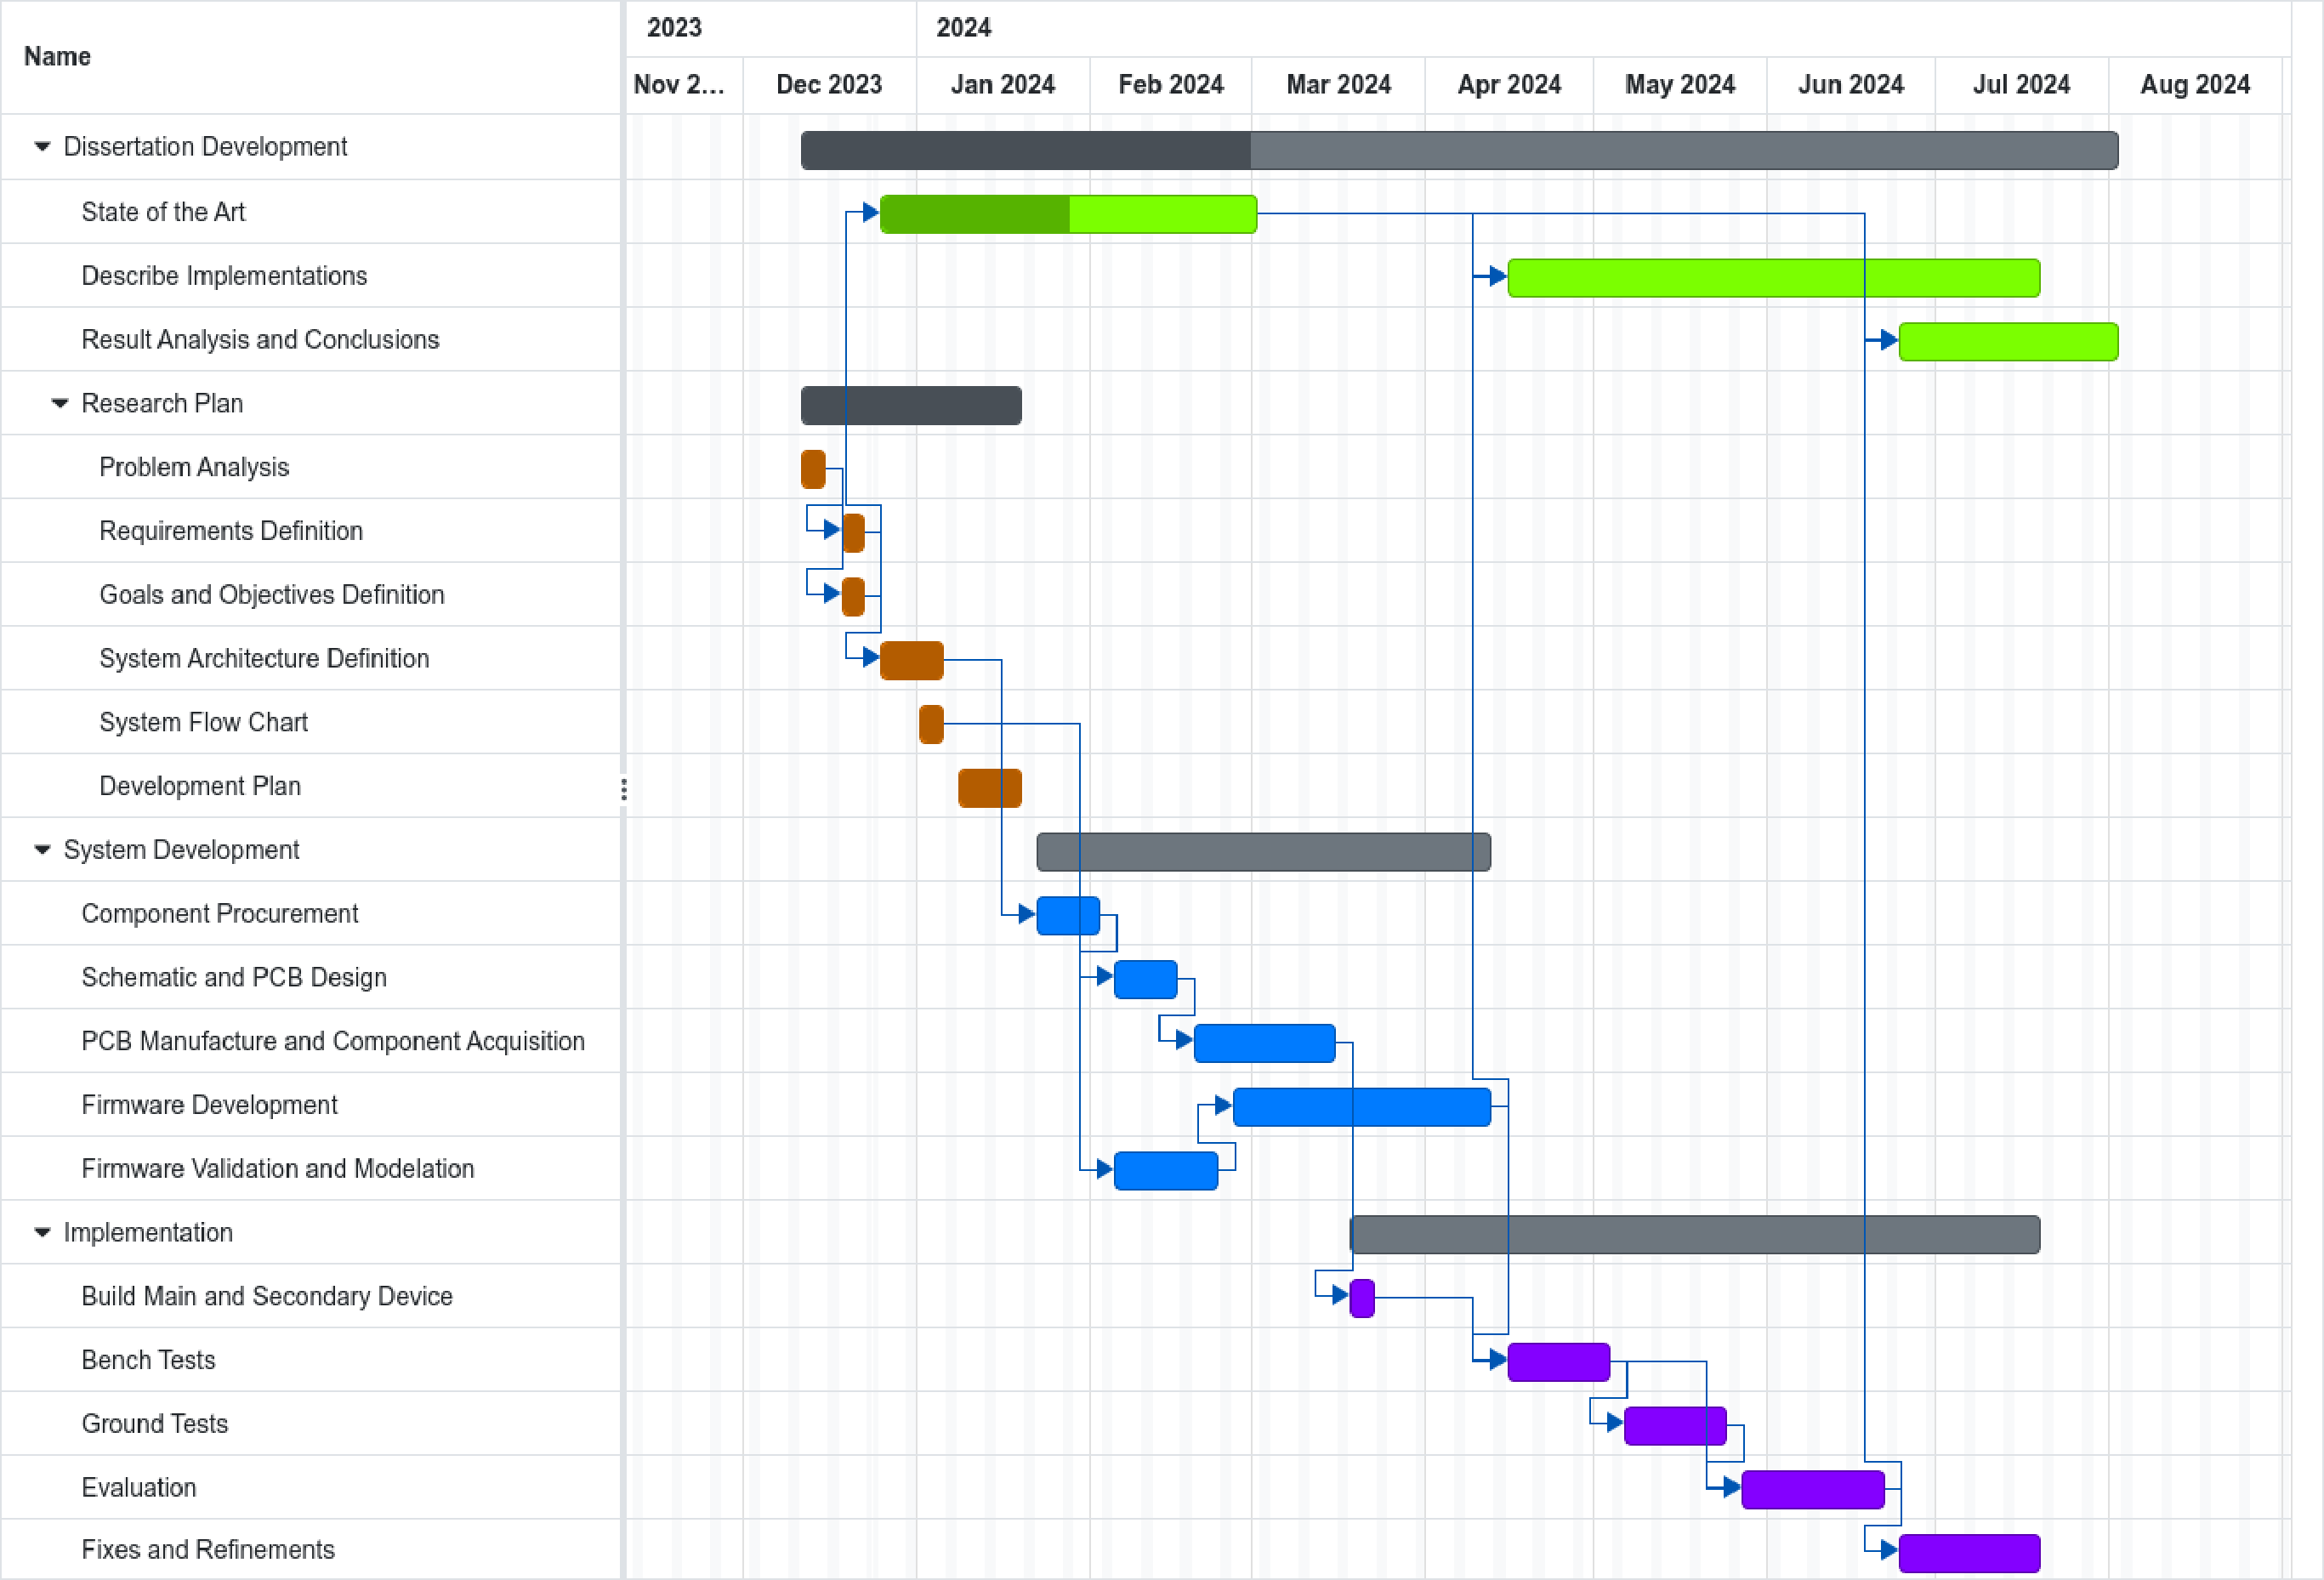
\includegraphics[width=\textwidth,keepaspectratio]{ch4/assets/gantt.pdf}
    \caption{Project timeline Gantt chart}
    \label{fig:gantt}
\end{figure}

The work load will be the following:
\begin{itemize}
    \item Dissertation Development - 170 days
    \item Research Plan - 30 days
    \item System Development - 60 days
    \item Hardware - 40 days
    \item Firmware - 50 days
    \item Implementation - 90 days
    \item Tests - 30 days
\end{itemize}

This timeline will help to ensure that all necessary activities are completed in the correct order and on time.
